\documentclass[11pt,a4paper]{article}
\usepackage{graphicx}
\usepackage{tcolorbox}
\usepackage{xcolor}
\usepackage{geometry}
\usepackage{tikz}
\geometry{margin=0.8in}

% Define colors
\definecolor{mlblue}{RGB}{31, 119, 180}
\definecolor{mlorange}{RGB}{255, 127, 14}
\definecolor{mlgreen}{RGB}{44, 160, 44}
\definecolor{mlred}{RGB}{214, 39, 40}
\definecolor{mlpurple}{RGB}{148, 103, 189}

\title{\Large\textbf{Discovery 6: Outliers \& Misfits}\\
\vspace{0.3em}
\normalsize Finding What Doesn't Belong}
\date{}

\begin{document}
\maketitle
\vspace{-2em}

\section*{Spot the Outliers}

\begin{center}
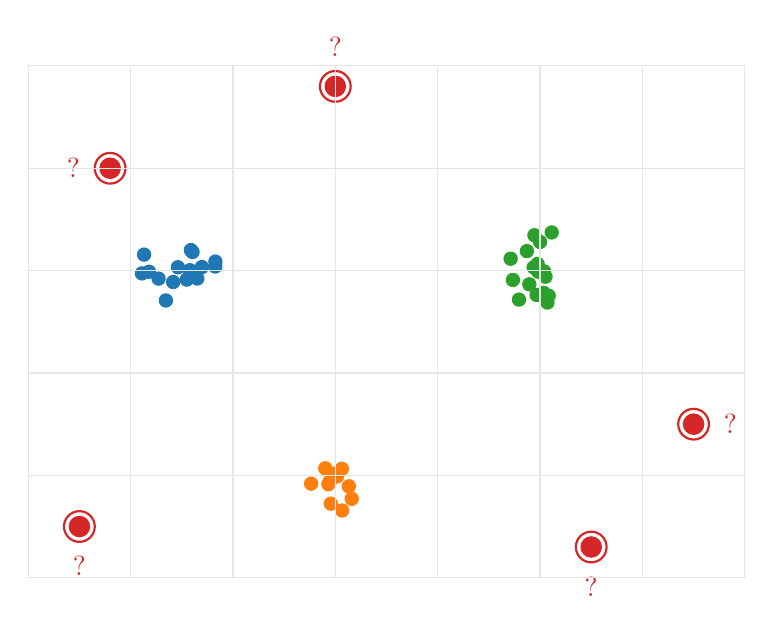
\begin{tikzpicture}[scale=1.3]
% Draw main clusters
% Cluster 1 - tight blue group
\foreach \i in {1,...,15} {
    \pgfmathsetmacro{\angle}{random(0,360)}
    \pgfmathsetmacro{\radius}{random(0,40)/100}
    \fill[mlblue] (1.5,3) ++(\angle:\radius) circle (2pt);
}

% Cluster 2 - tight green group
\foreach \i in {1,...,18} {
    \pgfmathsetmacro{\angle}{random(0,360)}
    \pgfmathsetmacro{\radius}{random(0,45)/100}
    \fill[mlgreen] (5,3) ++(\angle:\radius) circle (2pt);
}

% Cluster 3 - tight orange group
\foreach \i in {1,...,12} {
    \pgfmathsetmacro{\angle}{random(0,360)}
    \pgfmathsetmacro{\radius}{random(0,35)/100}
    \fill[mlorange] (3,1) ++(\angle:\radius) circle (2pt);
}

% OUTLIERS - make them stand out
\fill[mlred] (0.5,0.5) circle (3pt);
\draw[mlred, thick] (0.5,0.5) circle (0.15);
\node[mlred, below] at (0.5,0.3) {?};

\fill[mlred] (6.5,1.5) circle (3pt);
\draw[mlred, thick] (6.5,1.5) circle (0.15);
\node[mlred, right] at (6.7,1.5) {?};

\fill[mlred] (3,4.8) circle (3pt);
\draw[mlred, thick] (3,4.8) circle (0.15);
\node[mlred, above] at (3,5) {?};

\fill[mlred] (0.8,4) circle (3pt);
\draw[mlred, thick] (0.8,4) circle (0.15);
\node[mlred, left] at (0.6,4) {?};

\fill[mlred] (5.5,0.3) circle (3pt);
\draw[mlred, thick] (5.5,0.3) circle (0.15);
\node[mlred, below] at (5.5,0.1) {?};

% Grid
\draw[gray!20, thin] (0,0) grid (7,5);
\end{tikzpicture}
\end{center}

\vspace{0.5em}

\begin{tcolorbox}[colback=mlred!10, colframe=mlred!50]
\centering\Large
\textbf{Circle the dots that don't belong}
\end{tcolorbox}

\vspace{1.5em}

\section*{Three Types of Misfits}

\begin{center}
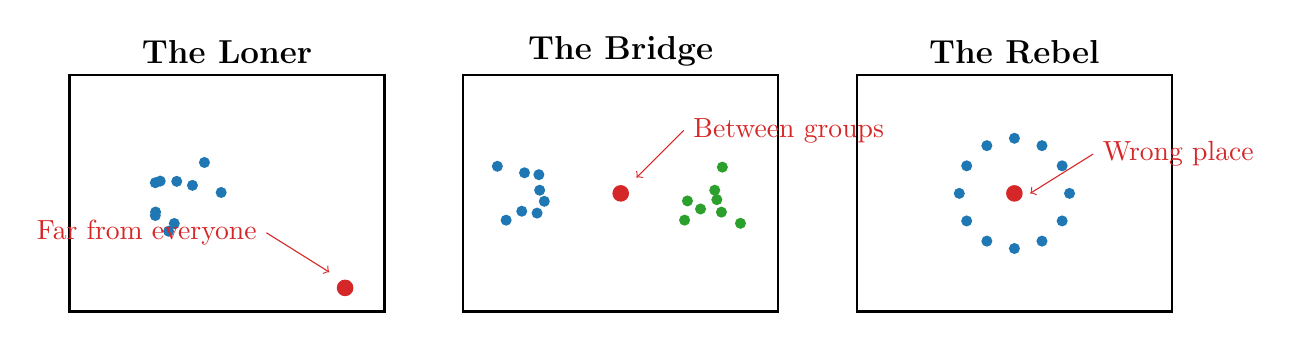
\begin{tikzpicture}[scale=1]
% The Loner
\begin{scope}[shift={(0,0)}]
\draw[thick] (0,0) rectangle (4,3);
\node[font=\large\bfseries] at (2,3.3) {The Loner};
\foreach \i in {1,...,10} {
    \pgfmathsetmacro{\x}{1.5 + rand*0.5}
    \pgfmathsetmacro{\y}{1.5 + rand*0.5}
    \fill[mlblue] (\x,\y) circle (2pt);
}
\fill[mlred] (3.5,0.3) circle (3pt);
\draw[mlred, <-] (3.3,0.5) -- (2.5,1) node[left] {Far from everyone};
\end{scope}

% The Bridge
\begin{scope}[shift={(5,0)}]
\draw[thick] (0,0) rectangle (4,3);
\node[font=\large\bfseries] at (2,3.3) {The Bridge};
\foreach \i in {1,...,8} {
    \pgfmathsetmacro{\x}{0.8 + rand*0.4}
    \pgfmathsetmacro{\y}{1.5 + rand*0.4}
    \fill[mlblue] (\x,\y) circle (2pt);
}
\foreach \i in {1,...,8} {
    \pgfmathsetmacro{\x}{3.2 + rand*0.4}
    \pgfmathsetmacro{\y}{1.5 + rand*0.4}
    \fill[mlgreen] (\x,\y) circle (2pt);
}
\fill[mlred] (2,1.5) circle (3pt);
\draw[mlred, <-] (2.2,1.7) -- (2.8,2.3) node[right] {Between groups};
\end{scope}

% The Rebel
\begin{scope}[shift={(10,0)}]
\draw[thick] (0,0) rectangle (4,3);
\node[font=\large\bfseries] at (2,3.3) {The Rebel};
\foreach \angle in {0,30,60,90,120,150,180,210,240,270,300,330} {
    \fill[mlblue] (2,1.5) ++(\angle:0.7) circle (2pt);
}
\fill[mlred] (2,1.5) circle (3pt);
\draw[mlred, <-] (2.2,1.5) -- (3,2) node[right] {Wrong place};
\end{scope}
\end{tikzpicture}
\end{center}

\newpage

\section*{Why Outliers Matter}

\begin{center}
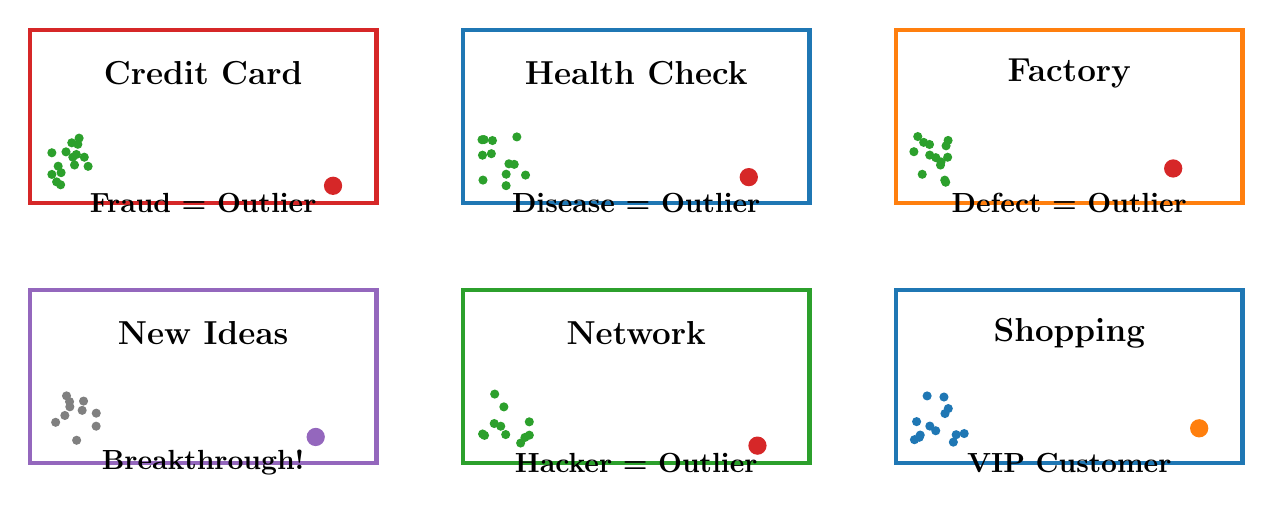
\begin{tikzpicture}[scale=1.1]
% Fraud detection
\draw[ultra thick, mlred] (0,5) rectangle (4,7);
\node[font=\large\bfseries] at (2,6.5) {Credit Card};
\foreach \i in {1,...,15} {
    \fill[mlgreen] (0.5+rand*0.3,5.5+rand*0.3) circle (1.5pt);
}
\fill[mlred] (3.5,5.2) circle (3pt);
\node at (2,5) {\textbf{Fraud = Outlier}};

% Medical diagnosis
\draw[ultra thick, mlblue] (5,5) rectangle (9,7);
\node[font=\large\bfseries] at (7,6.5) {Health Check};
\foreach \i in {1,...,12} {
    \fill[mlgreen] (5.5+rand*0.3,5.5+rand*0.3) circle (1.5pt);
}
\fill[mlred] (8.3,5.3) circle (3pt);
\node at (7,5) {\textbf{Disease = Outlier}};

% Quality control
\draw[ultra thick, mlorange] (10,5) rectangle (14,7);
\node[font=\large\bfseries] at (12,6.5) {Factory};
\foreach \i in {1,...,14} {
    \fill[mlgreen] (10.5+rand*0.3,5.5+rand*0.3) circle (1.5pt);
}
\fill[mlred] (13.2,5.4) circle (3pt);
\node at (12,5) {\textbf{Defect = Outlier}};

% Innovation
\draw[ultra thick, mlpurple] (0,2) rectangle (4,4);
\node[font=\large\bfseries] at (2,3.5) {New Ideas};
\foreach \i in {1,...,10} {
    \fill[gray] (0.5+rand*0.3,2.5+rand*0.3) circle (1.5pt);
}
\fill[mlpurple] (3.3,2.3) circle (3pt);
\node at (2,2) {\textbf{Breakthrough!}};

% Network security
\draw[ultra thick, mlgreen] (5,2) rectangle (9,4);
\node[font=\large\bfseries] at (7,3.5) {Network};
\foreach \i in {1,...,11} {
    \fill[mlgreen] (5.5+rand*0.3,2.5+rand*0.3) circle (1.5pt);
}
\fill[mlred] (8.4,2.2) circle (3pt);
\node at (7,2) {\textbf{Hacker = Outlier}};

% Customer behavior
\draw[ultra thick, mlblue] (10,2) rectangle (14,4);
\node[font=\large\bfseries] at (12,3.5) {Shopping};
\foreach \i in {1,...,13} {
    \fill[mlblue] (10.5+rand*0.3,2.5+rand*0.3) circle (1.5pt);
}
\fill[mlorange] (13.5,2.4) circle (3pt);
\node at (12,2) {\textbf{VIP Customer}};
\end{tikzpicture}
\end{center}

\vspace{1em}

\section*{Your Turn: Find Your Outliers}

\begin{center}
\Large\textbf{Think of your class/team/group}

\vspace{1em}

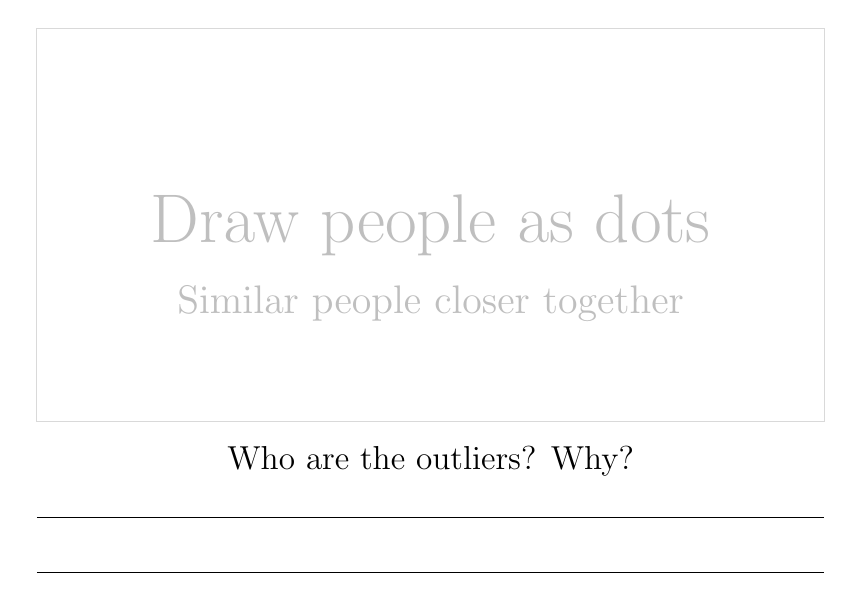
\begin{tikzpicture}[scale=1]
\draw[gray!30] (0,0) rectangle (10,5);
\node[gray!50] at (5,2.5) {\Huge Draw people as dots};
\node[gray!50] at (5,1.5) {\Large Similar people closer together};

\node at (5,-0.5) {\large Who are the outliers? Why?};
\node at (5,-1.2) {\underline{\hspace{10cm}}};
\node at (5,-1.9) {\underline{\hspace{10cm}}};
\end{tikzpicture}
\end{center}

\vspace{1em}

\section*{The Big Question}

\begin{center}
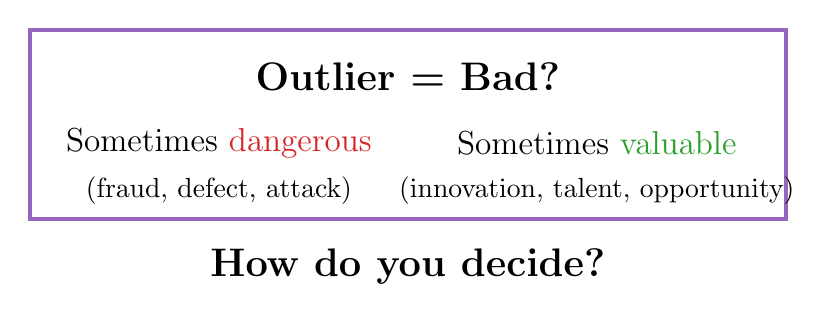
\begin{tikzpicture}[scale=1.2]
\draw[ultra thick, mlpurple] (0,0) rectangle (8,2);
\node at (4,1.5) {\Large\textbf{Outlier = Bad?}};
\node at (2,0.8) {\large Sometimes \textcolor{mlred}{dangerous}};
\node at (2,0.3) {(fraud, defect, attack)};
\node at (6,0.8) {\large Sometimes \textcolor{mlgreen}{valuable}};
\node at (6,0.3) {(innovation, talent, opportunity)};

\node at (4,-0.5) {\Large\textbf{How do you decide?}};
\end{tikzpicture}
\end{center}

\vspace{1em}

\begin{tcolorbox}[colback=mlpurple!10, colframe=mlpurple!50]
\centering\large
\textbf{Next Class:} How ML detects outliers automatically
\end{tcolorbox}

\end{document}